%%% Henrik Sopart, 836188, Latex-Projekt %%%% Version: Abgabe

\section[FPV-Drohnen]{FPV-Drohnen}
    \subsection[Besonderheiten]{Besonderheiten}
        FPV-Drohnen, auch bekannt als Racing- oder Freestyle-Drohnen  besitzen erhebliche Unterschiede
        im Vergleich zu handelsüblichen Drohnen wie beispielsweise der „DJI Mavic 3“. In der folgenden
        Tabelle werden die Unterschiede der beiden Typen gegenübergestellt. Im Anschluss wird genauer
        auf die Unterschiede in der Steuerung und der Komplexität eingegangen.

        \begin{table}[h]
            \renewcommand{\arraystretch}{1.5}
            \begin{tabular}{p{3cm}p{5.86cm}p{5.86cm}}
                \toprule
                \textbf{Merkmal} & \textbf{Handelsüblich} & \textbf{FPV} \\
                \midrule
                Steuerung                       & Unterstützungen durch Assistenzsysteme wie GPS oder Hinderniserkennung und vorprogrammierte Flugmodi~\cite{Mavic3DJI}                                                              & Im Normalfall keine Assistenzsysteme oder Flugmodi vorhanden \\
                Sichtverhältnisse               & Flug über Sichtlinie oder Bildschirm, welcher an der Fernsteuerung befestigt ist und das Videosignal empfängt                                                                     & Flug mit einer FPV-Brille, welche das Videosignal empfängt \\
                Verwendungszweck                & Fotografie, Videografie, Vermessungstechnik, Such- und Rettungsarbeiten, Landwirtschaft                                                                                           & Rennen, Wettbewerbe, Freestyle-Flüge, sehr dynamische Videografie \\
                Kamera                          & Meist eine mittels Gimbal stabilisierte Kamera, welche an der Unterseite der Drohne befestigt ist und sich nach oben und unten neigen lässt                                       & Meist zwei in einem festen Winkel montierte Kameras. Eine vorne im Rahmen, die das Bild zur FPV-Brille überträgt. Eine, die auf dem Rahmen befestigt wird und das Video aufnimmt (Actioncam) \\
                Akkulaufzeit                    & Meist deutlich höhere Akkulaufzeiten, beispielsweise bis zu 46 Minuten bei der Mavic 3~\cite{Mavic3DJI}                                                                            & Meist deutlich geringere Akkulaufzeit, beispielsweise 5\dq FPV-Drohne 4 bis 10 Minuten, abhängig von der Flugweise \\
                Geschwindigkeit und Agilität    & Geringere Geschwindigkeit und Agilität, die Mavic 3 ist beispielsweise auf \qty{75,6}{\kilo\metre\per\hour} und einem Nickwinkel von maximal 35 Grad beschränkt~\cite{Mavic3DJI}   & Hohe Geschwindigkeiten von weit über \qty{150}{\kilo\metre\per\hour} möglich, kein begrenzter Nickwinkel \\
                \bottomrule
            \end{tabular}
            \caption{Unterschiede}
            \label{tabelle_unterschiede}
        \end{table}

    \newpage
    \subsection[Steuerung]{Steuerung}
        Die Steuerung einer FPV-Drohne unterscheidet sich im Wesentlichen in zwei Punkten von der einer
        herkömmlichen. Zum einen bietet die FPV-Drohne im Normalfall keinerlei Assistenzsysteme, zum anderen
        ist die Reaktion der Drohne auf an der Fernsteuerung eingegebene Befehle eine andere. Sobald sich
        bei einer herkömmlichen Drohne beide Sticks der Fernsteuerung in der neutralen Position in der Mitte
        befinden, bleibt die Drohne in der Luft stehen. Wird nun der rechte Stick um das Maximale nach vorne
        bewegt, neigt sich die Drohne nach vorne und beschleunigt. Da die Neigung durch diverse Assistenzsysteme
        begrenzt ist, besteht kein Risiko, dass die Drohne „vorne überkippt“. Wird nun die Fernsteuerung
        losgelassen, bewegt sich der Stick wieder in die neutrale Position und die Drohne bleibt in der Luft
        stehen. Vereinfacht lässt sich sagen, dass die Bewegung am Stick in einen Neigungswinkel der Drohne resultiert.
        Die Leistung der Motoren wird automatisch angepasst, um (in diesem Beispiel) den Vorwärtsflug auf
        gleichbleibender Höhe zu ermöglichen. Die Höhe wird über den linken Stick kontrolliert. Allerdings
        geschieht dies relativ zur benötigten Drehzahl, um die Drohne in dieser Höhe zu halten. Befindet sich
        beispielsweise der linke Stick in der neutralen Position, drehen die Propeller so schnell, dass die
        Drohne weder sinkt noch steigt. Wird nun der Stick maximal nach vorne bzw. hinten betätigt, erhöht
        beziehungsweise verringert sich die Drehzahl der Motoren um einige Prozent, damit die Drohne langsam
        steigen beziehungsweise sinken kann. Bei einer herkömmlichen Drohne ist dementsprechend für keine Achse
        ein kontinuierliches Eingreifen durch den Piloten erforderlich. \\
        \\
        Im Vergleich hierzu würde eine FPV-Drohne, bei der der rechte Stick maximal nach vorne gedrückt wird,
        unkontrolliert nach „vorne kippen“ und sich um diese Achse drehen, bis es zum Absturz kommt. Zusätzlich
        gibt es bei FPV-Drohnen keine neutrale Stickposition, bei welcher die Drohne an der Stelle stehen bleibt.
        Jeder Befehl der Fernsteuerung wird ausgeführt. Vereinfacht bedeutet dies, dass eine Bewegung am Stick
        nicht in einem Winkel, sondern in einer Drehgeschwindigkeit um die gesteuerte Achse resultiert. Auch die
        Höhensteuerung funktioniert anders als bei einer herkömmlichen Drohne. Am einfachsten lässt sich dies mit
        einem Potenziometer vergleichen. Befindet sich der linke Stick ganz hinten, drehen die Propeller nicht.
        Wird diese nun nach vorne bewegt, erhöht sich die Drehzahl bis auf den maximalen Wert. Wird die Fernsteuerung
        nun losgelassen, behält die Drohne diese Drehzahl bzw. Drehgeschwindigkeit bei. Da die Bewegung einer Achse
        nur durch direktes Eingreifen des Piloten zu stoppen ist und diese Bewegung nicht wie bei einer herkömmlichen
        Drohne weitere Achsen ansteuert, um beispielsweise einen Vorwärtsflug mit gleichbleibender Höhe zu ermöglichen,
        ist ein kontinuierliches Eingreifen durch den Piloten zwingend erforderlich.
        
    \newpage       
    \subsection[Komplexität]{Komplexität}
        Da die meisten herkömmlichen Drohnen für eine große Zielgruppe entwickelt wurden, sind keine technischen
        Fähigkeiten oder Vorkenntnisse erforderlich, um mit einer solchen Drohne Luftaufnahmen zu erstellen~\cite{shon2022}.
        Durch das Zusammenspiel unterschiedlichster Sensoren, wie beispielsweise eine Hinderniserkennung und GPS,
        wird das Risiko für die Drohne minimiert. Zusätzlich erleichtern es Technologien wie Geofencing dem Piloten,
        innerhalb der rechtlichen Grenzen zu fliegen. \\
        \\
        Da FPV-Drohnen immer populärer werden, haben sich in den letzten Jahren neue Möglichkeiten gefunden, in
        dieses Hobby einzusteigen. Seit 2021 bietet die Firma „DJI“ zwei FPV-Drohnen an. Diese müssen nicht selbst
        zusammengebaut werden und erfordern ähnlich wie herkömmliche Drohnen keinerlei technische Fähigkeiten oder
        Vorkenntnisse~\cite{DJIAvatar}\cite{DJIFpv}. Da diese Drohnen jedoch proprietäre Komponenten verwenden, auf welche der Käufer keinen Einfluss
        hat, wird auf diese im weiteren Verlauf dieser Arbeit nicht weiter eingegangen. \\
        \\
        Bis vor einigen Jahren gab es nur die Möglichkeit, sämtliche Komponenten wie beispielsweise Motoren,
        Controller, Kamera oder den Rahmen einzeln zu kaufen und sich so seine eigene Drohne zu bauen. Dies
        erfordert ein hohes Maß an technischem Wissen und technischen Fähigkeiten, jedoch erhält man die Möglichkeit,
        die Drohne individuell auf die Bedürfnisse des Piloten anzupassen. Beispielsweise würde für eine Drohne,
        welche Aufnahmen in den Alpen anfertigen soll die Akkulaufzeit eine Priorität sein und aus diesem Grunde
        schwächere, aber effizientere Motoren zum Einsatz kommen. Hingegen würde eine Drohne, welche Autos
        auf einer Rennstrecke verfolgt, leistungsstarke Motoren erhalten. \\
        \\
        In der folgenden Abbildungen werden die oben beschriebenen Unterschiede sichtbar. In Abbildung~\ref*{HandelsueblicheDrohne}
        ist eine handelsübliche Drohne zu sehen, in Abbildung~\ref*{FpvDrohne} eine FPV-Drohne.

        \vspace{1.2cm}
        \begin{figure}[h]
            \centering
            \begin{subfigure}[b]{0.45\textwidth}
                \centering
                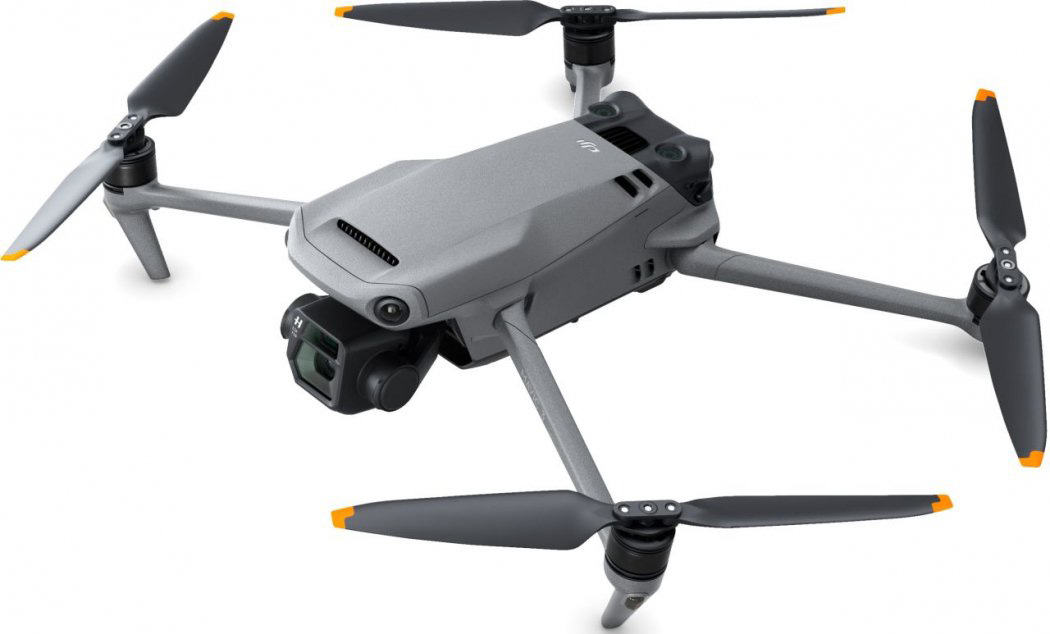
\includegraphics[width=\textwidth]{Img/Bild_DJIMavic3.jpg}
                \caption{Handelsübliche Drohne: DJI Mavic 3~\cite{BildMavic3}}
                \label{HandelsueblicheDrohne}
            \end{subfigure}
            \hfill
            \begin{subfigure}[b]{0.45\textwidth}
                \centering
                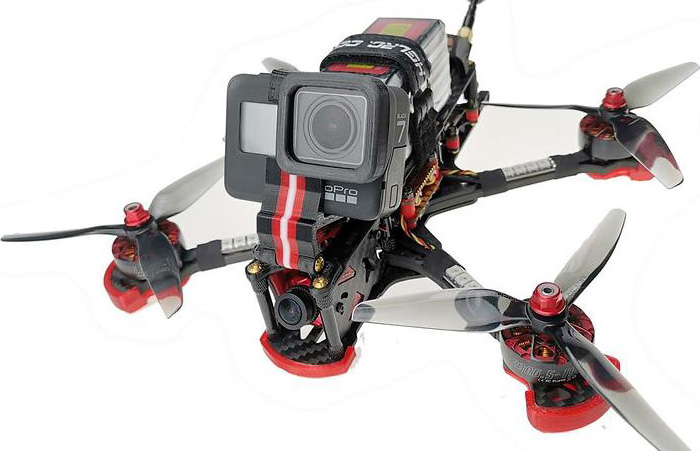
\includegraphics[width=\textwidth]{Img/Bild_FPV.jpg}
                \caption{FPV-Drohne: HGLRC FPV Sector 5 V3~\cite{BildFpv}}
                \label{FpvDrohne}
            \end{subfigure}
               \caption{Beispielbilder}
               \label{BeispielBilder}
       \end{figure}